\chapter{Opdracht}

\section{Introductie}

Het bedrijf Shop2market is een software development bedrijf in de business-to-business sector. De organisatie helpt webwinkels online adverteren met als doelstelling de winstgevendheid van online advertenties te maximaliseren. Shop2market is ontstaan nadat duidelijk werd dat veel bedrijven niet de technologische middelen of kennis in huis hebben om zelfstandig te kunnen starten met adverteren. Zo blijkt uit interactie met klanten dat velen vrezen voor hoge kosten. Volgens mede opdrichter van Shop2market Matthijs Jorissen, komt dit door het gebrek aan transparantie en het complexe landschap dat is gecreeërd door de grootte hoeveelheid bedrijven.

Voor alsnog diende shop2market als een IT oplossing ondersteunend aan het adviesbedrijf. Het merendeel van deze klanten zijn webwinkels in het A segment. Maar omdat de integratie met een webwinkel vaak maatwerk opleverde duurde een integratie gemiddeld zes tot acht maanden. Dit heeft een hoop klanten opgeleverd maar bleef erg onderhoudsintensief en hinderde de groei van Shop2market.

Hierdoor heeft het bedrijf zijn strategie opnieuw gedefinieerd. Hieruit kwam dat het webwinkels in het midden en klein bedrijf op internationaal niveau wil kunnen bedienen. De gewenste groei moet mogelijk worden gemaakt doordat webwinkel platformen zoals SEOShop, Shopify en Magento een gestandaardiseerde integratie mogelijk maken. Hierdoor wordt een webwinkel geïntegreerd in slechts enkele minuten.

Adcurve is een online dienst die is ontwikkeld in 2015 door Shop2market. Met de ervaring vanuit de adviesorganisatie zijn veel processen vertaald naar functionaliteiten om een self-service applicatie mogelijk te maken. De eerste beta versie van Adcurve is in de zomer van 2015 gelanceerd voor webwinkels die gebruik maken webwinkelplatformen als SEOshop of Magento. Hiermee kunnen webwinkels volledig zelfstandig aan de slag.

Webwinkel eigenaren kunnen nu hun producten gemakkelijk adverteren via zogeheten publishers. Dit zijn bedrijven die de advertenties publiseren. Bijvoorbeeld ingekochte zoekresultaten op Google via Google Adwords, op prijsvergelijkers en affiliate via Beslist.nl of Zanox. Maar ook Marktplaatsen zoals Amazon.com en Google Shopping maken hier onderdeel van uit.

Vervolgens biedt Adcurve de mogelijkheid om de impact van de advertenties in te zien en te handelen aan de hand van de winstgevendheid. Dit is mogelijk doordat Adcurve een partij is tussen de webwinkel en geinstalleerde publishers. Er vindt een volledige integratie plaats waarbij de afkomstigheid van bezoekers, bestellingen word gemeten. In combinatie met de advertentiekosten van publishers worden de nodige statistieken berekend.

Omdat de belangrijkste functionaliteiten zijn gebaseerd op statistieken is het belangrijk dat statistieken op tijd zijn berekend, beschikbaar zijn.
Om een goede gebruikers-ervaring te bieden is er een toenemende wens om de huidige oplossing te herzien. De scriptie hier verder op in gaan en onderzoeken hoe de gestelde doelstellingen behaald kunnen worden.


\section{Aanleiding} % de aanleiding tot de opdracht

\begin{figure}[h]
    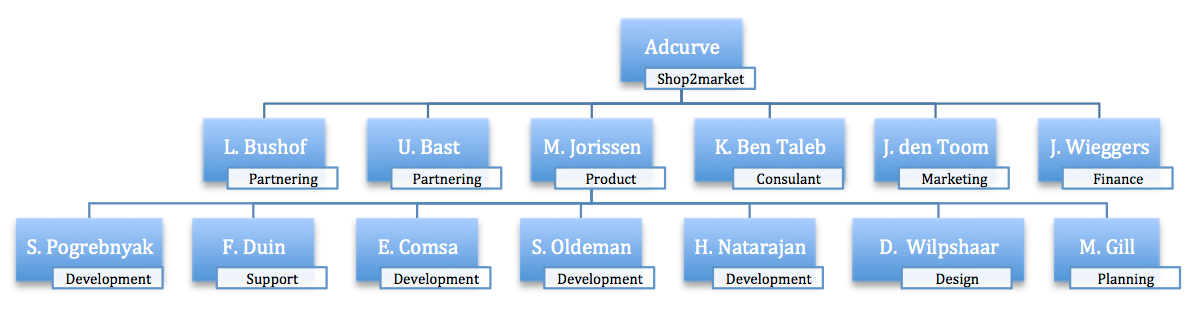
\includegraphics[width=1\textwidth]{organisation_structure.png}
    \caption{Organogram waarin de relatie tussen Shop2market en Adcurve zichtbaar is.}
    \label{fig:orgchart}
\end{figure}

\section{Context van het bedrijf} % de op te leveren producten met kwaliteitscriteria;


\section{De kwestie} % een kwestie (aanleiding, het op te lossen probleem, de te vervullen behoefte of de te benutten kans);

\section{Doelstellingen} % de doelstellingen (wat moet na afloop van het afstudeerproject zijn bereikt);

\section{Deel producten}


% TODO: Het type opdracht kan worden omschreven als een product en ontwerp opdracht. 


